\label{pagcap3}
\chapter{Optimizaci�n e implementaci\'on de multiprocesamiento}
%OSO ATENCION - FIJARSE QUE SEA CONSISTENTE LA NOMENCLATURA DE FIGURAS. SE PONE SIEMPRE "Fig. X", no fig X, Fig X, figura X, imagen X, etc.

\section{Introducci\'on}
En los cap\'itulos anteriores presentamos la problem\'atica por la cual surge la idea y la necesidad de paralelizar la programaci\'on, as\'i como las herramientas a utilizar, en nuestro caso OpenMP bajo Fortran. La elecci\'on del lenguaje Fortran se debe a que el usuario de la aplicaci\'on utilizada es tambi\'en su creador, de manera que, para hacer el cambio lo m\'as transparente posible, se decide no alterar este aspecto del programa.

Con Fortran como base, y teniendo en cuenta la estructura del programa con un an\'alisis inicial del mismo, debido a las caracter\'isticas de programa estructurado, monol\'itico y no modularizado, se elige orientar la soluci\'on a aplicar concurrencia en un entorno de Memoria Compartida y dejar habilitada la ejecuci\'on paralela en un equipo multiprocesador.

La aplicaci\'on bajo estudio utiliza archivos de datos en disco para guardar resultados, tanto parciales como finales. Esta actividad de entrada/salida introduce importantes demoras en el tiempo de respuesta, que necesitamos considerar. En este cap\'itulo describiremos el proceso seguido para la optimizaci\'on del c\'odigo Fortran en lo relacionado con el manejo de los archivos. Esta primera fase de optimizaci\'on permitir\'a la paralelizaci\'on de segmentos de c\'odigo.

Tambi\'en realizaremos un an\'alisis del perfil de ejecuci\'on de la aplicaci\'on con una herramienta de perfilado  que permitir\'a identificar qu\'e subrutinas son las que m\'as tiempo consumen y cu\'ales son las m\'as indicadas para aplicar la paralelizaci\'on.

Por \'ultimo veremos la forma como se ha aplicado OpenMP a las partes seleccionadas de la aplicaci\'on. Explicaremos por qu\'e han sido seleccionadas ciertas construcciones espec\'ificas del c\'odigo y las razones de modificar algunas estructuras de control para hacer m\'as eficiente la utilizaci\'on de la memoria y de la CPU.


\section{An\'alisis de la aplicaci\'on}
Primero se analiz\'o la aplicaci\'on para poder proceder con su optimizaci\'on y paralelizaci\'on. Como se explic\'o  en la secci\'on \ref{sec:n6}, determinamos la plataforma en que deber\'ia ejecutarse la aplicaci\'on, estableciendo versi\'on de sistema operativo  y arquitectura. La aplicaci\'on recibida fue utilizada por su programador, en arquitectura x86 de 32 bits, bajo sistema operativo GNU/Linux, espec\'ificamente con la distribuci\'on CentOS. 

Lo primero fue obtener resultados base de ejecuciones de la aplicaci\'on bajo ese entorno, a fin de tener una referencia para la comparaci\'on de resultados. El autor de la aplicaci\'on nos indic\'o que la misma es completamente determin\'istica, con lo cual la aplicaci\'on, con los mismos datos de entrada provistos, debe arrojar los mismos resultados en todas las ejecuciones. 

Para llevar a cabo el trabajo de la Tesis se seleccion\'o el entorno GNU/Linux, con la distribuci\'on Slackware de 64 bits como base, a la cual no fue necesario agregar componentes ni efectuar ninguna compilaci\'on especial. Se verific\'o que la aplicaci\'on entregada por el usuario compilara correctamente sin ninguna modificaci\'on en esta plataforma y arrojara, para los datos de entrada, exactamente los mismos resultados que en su entorno original. 

Con esto ya verificado se avanz\'o en el trabajo de Tesis hacia el an\'alisis propiamente dicho de la aplicaci\'on. 

Como vimos en el cap\'itulo anterior, lo primero antes de optimizar es tener una aplicaci\'on que produzca resultados correctos. En nuestro caso se nos present\'o una aplicaci\'on ya depurada y funcionando correctamente, por lo cual no debimos preocuparnos por esta parte, as\'i que pasamos a la parte de optimizaci\'on, donde se deben seleccionar previamente los casos de test para validar que la optimizaci\'on sigue produciendo resultados correctos.

Contamos con dos casos de test provistos por el creador de la aplicaci\'on, los cuales se identifican por dos par\'ametros (nr y no) que definen, respectivamente, la cantidad total de palas y de nodos sobre los cuales se va a realizar la simulaci\'on. Con estos par\'ametros se definen los casos de test, con valores iguales para ambos datos: nr = no = 50 en el primer caso de test, y nr = no = 80 en el segundo caso.

Estos valores tambi\'en definen unas variables globales comunes de la aplicaci\'on llamadas ``maxir'' y ``maxio'' que se fijan a nr+1 y no+1 respectivamente. Los valores est\'an codificados directamente en la aplicaci\'on y no se utiliza ning\'un tipo de constante simb\'olica que los defina, algo que ser\'ia m\'as adecuado para el tratamiento de dichos valores y para tener un c\'odigo m\'as limpio; esto no se modific\'o y se mantuvo el tratamiento original de los valores para alterar lo menos posible el c\'odigo. 

Por el mismo motivo, tampoco se modific\'o la obtenci\'on de los valores de entrada para las simulaciones a partir de un archivo de texto.

\subsection{An\'alisis de perfilado}\label{ssec:perfilado}
Como paso preliminar de la optimizaci\'on realizamos an\'alisis de la aplicaci\'on con la herramienta de perfilado gprof, para poder comparar los principales puntos de consumo de tiempo con anterioridad a la optimizaci\'on y luego de la misma. De esta forma se pretende seleccionar una o varias subrutinas para la paralelizaci\'on y observar de qu\'e manera cambia el comportamiento de la aplicaci\'on con la optimizaci\'on.

Los datos obtenidos mediante gprof en esta etapa muestran que la subrutina ``estela'' resulta ser la que consume el mayor porcentaje, 79,83\% del tiempo de ejecuci\'on de la aplicaci\'on. Le sigue la subrutina ``solgauss'' con un 14,36\%. Estos datos se pueden observar en la Fig. \ref{figGprof1}.

\begin{figure}[h!]%[htp]
  \centering
  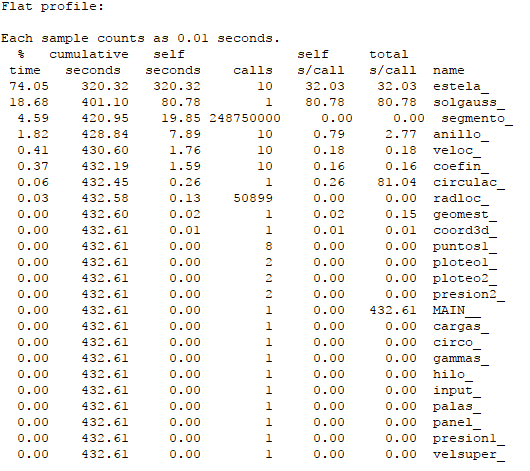
\includegraphics[width=0.60\textwidth]{figuras/gprof1.png} \\
  \caption{Salida de \emph{gprof} en el primer equipo.} %
   \label{figGprof1}
\end{figure}

Con estos resultados se pudo inferir en esta primer revisi\'on que estas dos subrutinas son las candidatas a ser optimizadas con procesamiento paralelo.

Para las pruebas se utilizaron dos computadoras de escritorio distintas, ambas multiprocesadores. El primer equipo posee un procesador AMD Phenom II con 4 nucleos y 4GB de memoria RAM. El segundo equipo consta de un procesador Intel Core i3 con 2 n\'ucleos (2 hilos cada procesador) y 6 Gb de RAM. Las especificaciones completas son provistas en el Cap\'itulo 4 donde se analizan los resultados obtenidos.

La salida de la Fig. \ref{figGprof1} fue obtenida en el primer equipo. Realizamos el mismo an\'alisis de perfilado sobre el segundo equipo, y observamos que la mayor porci\'on del tiempo sigue siendo consumida por la subrutina ``estela'' seguida por ``solgauss'' casi en los mismos porcentajes, 74,26\% y 16,84\% respectivamente. Tambi\'en es de notar la mejora en los tiempos de ejecuci\'on. Esto se puede observar en la Fig. \ref{figGprof2}.

\begin{figure}[h!]%[htp]
  \centering
  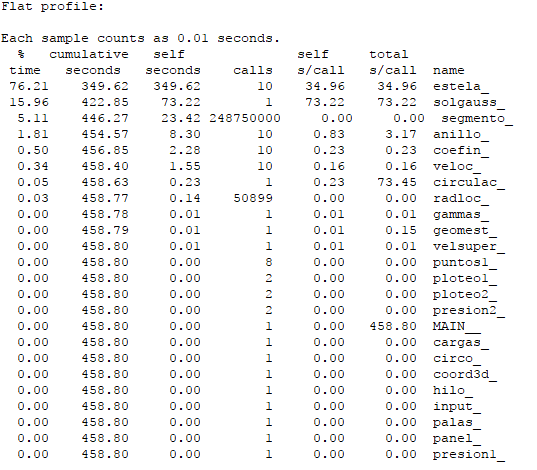
\includegraphics[width=0.60\textwidth]{figuras/gprof2.png} \\
  \caption{Salida de \emph{gprof} en el segundo equipo.} %
   \label{figGprof2}
\end{figure}

A esta altura del trabajo contamos con ``c\'odigo correcto no optimizado'' (Unoptimized Correct Code)\citep{Garg}, de modo que, siguiendo las etapas del proceso de optimizaci\'on (ilustradas en \ref{figGySEtapas}) visto en el cap\'itulo 2, debemos efectuar una optimizaci\'on serial para obtener c\'odigo optimizado. Luego de esto podremos pasar a la etapa de ``Optimizaci\'on Paralela'', donde aplicaremos paralelizaci\'on al c\'odigo para obtener justamente c\'odigo paralelo optimizado. 

En las siguientes secciones veremos c\'omo realizamos estas dos etapas del proceso para obtener nuestra aplicaci\'on de estudio en forma optimizada paralela.

\section{Optimizaci\'on Serial del c\'odigo Fortran}
La optimizaci\'on serial es ``un proceso iterativo que involucra medir repetidamente un programa seguido de optimizar sus porciones cr\'iticas''\citep{Garg}. Obtenidas las mediciones iniciales del comportamiento, debemos optimizar las opciones de compilaci\'on y vincular  el c\'odigo objeto con bibliotecas optimizadas. En el trabajo de tesis intentamos reducir al m\'inimo las modificaciones al c\'odigo, por lo cual las opciones que se utilizar\'an para la compilaci\'on ser\'an \'unicamente las referidas a la infraestructura de programaci\'on paralela de OpenMP. 

Por lo dem\'as, la aplicaci\'on no hace uso de ninguna otra biblioteca que no se cuente entre las que utiliza regularmente el compilador para construir la aplicaci\'on. Como buscamos observar el impacto de optimizar serialmente el c\'odigo y aplicar paralelizaci\'on, no se utilizan bibliotecas que pudieran optimizar otras partes del programa.

\subsection{An\'alisis del acceso a datos de la aplicaci\'on}
Al analizar los resultados de ejecuci\'on de la aplicaci\'on observamos que maneja gran cantidad de archivos en disco, tanto de texto como binarios (temporales). En el directorio de la aplicaci\'on aparecen 34 archivos de extensi\'on TXT, 9 archivos PLT, 5 archivos OUT y 8 archivos TMP. A \'estos se agregan el propio archivo fuente .for, el ejecutable invisidosExe, el archivo con los datos de entrada entvis2f.in, y el que utilizamos para almacenar los datos de gprof, invisidosExegprof. En la Fig. \ref{consLS} se puede observar el listado del directorio de ejecuci\'on.\\
\begin{figure}[h!]%[htp]
  \begin{lstlisting}[style=consola, numbers=none]
        h4ndr3s@gondolin:~/pruebas/oldone\$ ls
        alfa.txt    	cp2.txt      	integ1.txt         	vel02int.txt
        arco.txt    	cpei.plt     	integ2.txt         	vel02pvn.txt
        cindg.tmp   	cpei.txt     	invisidos2fin.for  	   velcapae.txt
        circo.txt   	cr.txt       	invisidosExe*           velcapai.txt
        cix1.tmp    	entvis2f.in  	invisidosExegprof       velindad.plt
        cix2.tmp    	estel1.txt   	palas.plt          	velindad.txt
        ciy1.tmp    	estel2.txt   	palest.plt         	velpotad.txt
        ciy2.tmp    	estel3.txt   	panel.plt          	velresad.plt
        ciz1.tmp    	fuerza.plt   	panel.txt          	veltotal.txt
        ciz2.tmp    	fzas.txt     	pres.plt           	velxyz.txt
        co.txt      	gama.txt     	salida2.out        	vix.txt
        coefg.tmp   	gdifo.out    	subr.out           	viy.txt
        coefp.txt   	gdifr.out    	vector.plt         	viz.txt
        coord.txt   	gmon.out     	vel01ext.txt       	vn.txt
        cp075c.txt  	go.out       	vel01int.txt
        cp1.txt     	gr.out       	vel02ext.txt
  \end{lstlisting}
  \caption{Listado del directorio luego de la ejecuci\'on del programa}
  \label{consLS}
\end{figure}
Los tama\~nos de la mayor\'ia de los archivos van desde 8 KB hasta 2 MB, pero los archivos TMP pueden alcanzar un tama\~no de varios megabytes (se observan algunos del orden de los cientos de megabytes). Esto evidencia que una corrida de la aplicaci\'on intercambia un volumen significativo de datos entre la aplicaci\'on y el sistema de archivos.

Con el fin de localizar los puntos de aplicaci\'on de la optimizaci\'on, relevamos la relaci\'on entre cada archivo y las subrutinas que lo acceden, indicando las operaciones realizadas (escritura, lectura, lectura/escritura, rewind). De este relevamiento se obtiene la lista de archivos que \'unicamente son escritos en disco, y los que son adem\'as le\'idos, por cada subrutina. La relaci\'on de archivos y subrutinas se muestra en la tabla \ref{tab:tabArch}.\\

\begin{table}[htb]
\begin{center}
\begin{tabular}{|c|c|c|}
\hline 
\rule[-1ex]{0pt}{2.5ex} Archivos & Funci\'on & Operaci\'on \\ 
\hline 
\hline
\rule[-1ex]{0pt}{2.5ex} cpei.plt, cpei.txt & presion2 & write only \\ 
\hline 
\rule[-1ex]{0pt}{2.5ex} palest.plt & palas, geomest & write only \\ 
\hline 
\rule[-1ex]{0pt}{2.5ex} palas.plt, alfa.txt, coord.txt & palas & write only \\ 
\hline 
\rule[-1ex]{0pt}{2.5ex} panel.plt, panel.txt & panel & write only \\ 
\hline 
\rule[-1ex]{0pt}{2.5ex} pres.plt, cp075c.txt, coefp.txt, & presion1 & write only \\ 
%\hline 
\rule[-1ex]{0pt}{2.5ex}  cp1.txt, cp2.txt &  &  \\ 
\hline 
\rule[-1ex]{0pt}{2.5ex} velxyz.txt, velpotad.txt, velindad.txt &  & \\ 
%\hline 
\rule[-1ex]{0pt}{2.5ex} velcapae.txt, velcapai.txt, vix.txt & veloc & write only \\ 
%\hline 
\rule[-1ex]{0pt}{2.5ex} viy.txt, viz.txt &  &  \\ 
\hline 
\rule[-1ex]{0pt}{2.5ex} estel1.txt, estel2.txt, estel3.txt & geomest & write only \\ 
\hline 
\rule[-1ex]{0pt}{2.5ex} \multirow{2}{1cm}{gama.txt} & circulac & write only \\ \cline{2-3}
& gammas & read only \\ \cline{1-3} 
\hline 
\rule[-1ex]{0pt}{2.5ex} veltotal.txt, vel01ext.txt, vel01int.txt & velsuper & write only \\ 
%\hline 
\rule[-1ex]{0pt}{2.5ex} vel02ext.txt, vel02int.txt, vel02pvn.txt &  &  \\ 
\hline 
\rule[-1ex]{0pt}{2.5ex} velresad.plt & ploteo2 & write only \\ 
\hline 
\rule[-1ex]{0pt}{2.5ex} \multirow{2}{1cm}{arco.txt} & circulac & write only \\ \cline{2-3} 
& circo & read only \\ \cline{2-3}
\hline 
\rule[-1ex]{0pt}{2.5ex} fzas.txt, fuerza.plt, vector.plt & cargas & write only \\ 
\hline 
\rule[-1ex]{0pt}{2.5ex} \multirow{2}{1cm}{coefg.tmp, cindg.tmp} & circulac & write y rewind \\ \cline{2-3}
& solgauss & read y rewind \\ \cline{2-3}
\hline 
\rule[-1ex]{0pt}{2.5ex} \multirow{2}{1cm}{cix1.tmp, ciy1.tmp, ciz1.tmp} & anillo & write y rewind \\ \cline{2-3}
& coefin & read y rewind \\ \cline{2-3}
& - & - \\ \cline{2-3}
\hline 
\rule[-1ex]{0pt}{2.5ex} \multirow{3}{1cm}{cix2.tmp, ciy2.tmp, ciz2.tmp} & coefin & write y rewind \\ \cline{2-3} 
& circulac & read y rewind \\ \cline{2-3}
& veloc & read y rewind \\ \cline{2-3}
\hline 
\rule[-1ex]{0pt}{2.5ex} \multirow{4}{1cm}{salida2.out} & input & write only \\ \cline{2-3}
& cargas & write only \\ \cline{2-3}
& anillo & write only \\ \cline{2-3}
& veloc & write only \\ \cline{2-3}
%\hline 
\hline 
\end{tabular} 
\caption {Relaci\'on archivos y funciones de la aplicaci\'on}
\label{tab:tabArch}
\end{center}
\end{table}

Fortran ofrece los archivos regulares, o archivos externos soportados en disco (External Files), pero tambi\'en los archivos internos o Internal Files, que son cadenas de caracteres o arreglos de cadenas de caracteres, localizados en memoria principal. Los Internal Files se manejan con las mismas funciones que los archivos externos, y la \'unica restricci\'on para su uso es la cantidad de memoria virtual del sistema. 
Como la latencia de los accesos a disco magn\'etico es, normalmente, al menos cinco \'ordenes de magnitud mayor que la de los accesos a memoria principal\citep{Gregg}, cambiando la definici\'on de los archivos en disco a Internal Files (siempre que la restricci\'on de tama\~no del sistema de memoria virtual lo permita) conseguimos una mejora sustancial de performance de la aplicaci\'on, sin ninguna modificaci\'on importante al c\'odigo ni al comportamiento del programa.

\subsection{Optimizaci\'on por adaptaci\'on de archivos externos a internos}
La primera decisi\'on tomada para la optimizaci\'on del c\'odigo es reducir el impacto de los accesos a archivos en disco que son le\'idos y adem\'as escritos por la aplicaci\'on. No efectuaremos ninguna modificaci\'on sobre los archivos que son \'unicamente escritos por las subrutinas, con cuatro excepciones: la escritura de los archivos integ1.txt e integ2.txt en la subrutina estela, retrasada hasta el final de la misma, y los archivos salida2.out, que guarda resultados de la ejecuci\'on a medida que avanza, y subr.out, que recoge lo mostrado en salida est\'andar. 
Estos archivos se guardar\'an en objetos de tipo Internal File de Fortran y su escritura se demorar\'a hasta la finalizaci\'on del programa. La elecci\'on de no pasar m�s archivos a Internal Files es para evitar un incremento elevado en la cantidad de memoria utilizada por la aplicaci\'on.
%OSO POR QUE? %HANDRU por lo indicado m�s adelante, ocupar m�s memoria con m�s archivos
Un caso especial es el Internal File \emph{outstd} que lleva lo impreso en salida est\'andar dentro de algunas subrutinas(estela, geomest, etc), y es mostrado por pantalla al retornar dichas subrutinas al programa principal.

Luego, todo archivo o External File que sea escrito y le\'ido durante la ejecuci\'on de la aplicaci\'on ser\'a mantenido por un Internal File. La \'unica modificaci\'on necesaria al c\'odigo ser\'a el cambio de las referencias a los archivos en las sentencias ``write'', ``read'' y ``rewind''. En la Fig. \ref{codSinMod} se muestra un ejemplo de c\'odigo previo a la modificaci\'on, y en la Fig. \ref{codModif} el c\'odigo ya modificado.\\

\begin{figure}[htb]%[htp]
%  \begin{lstlisting}[style=For, numbers=none]
   \begin{BVerbatim}
      open(unit=15,file='subr.out')
      ...
      write(15,1)
      write(6,1)
   \end{BVerbatim}
%  \end{lstlisting}
  \caption{Ejemplo de c\'odigo sin modificar}
  \label{codSinMod}
\end{figure}


Como se ve, reemplazamos el archivo ``subr.out'' representado por el identificador de unidad 15 por el Internal File denominado subrout.

\begin{figure}[htb]%[htp]
%  \begin{lstlisting}[style=For, numbers=none]
   \begin{BVerbatim}
      character subrout(500)*60   ! Internal File
      ...
      write(subrout(nsubr),1)
      nsubr=nsubr+1
    !      write(15,1)
      write(6,1)
   \end{BVerbatim}
%  \end{lstlisting}
  \caption{Ejemplo de c\'odigo modificado para utilizar Internal File}
  \label{codModif}
\end{figure}

Como se ha dicho, el External File subr.out pasa a ser manejado como un Internal File, que como se ve en la declaraci\'on de la Fig. \ref{codModif}, es un arreglo de 500 cadenas de 60 caracteres como m\'aximo. La variable nsubr mantiene la posici\'on en el internal file a ser escrita, y el argumento ``1'' en los comandos write es un formato de escritura definido dentro del programa como se explicaba en el cap\'itulo anterior.
En la tabla \ref{tab:tabEquiv} vemos c\'omo quedan las equivalencias de los External Files y su correspondiente cambio a Internal File.

\begin{table}[htb]
\begin{center}
\begin{tabular}{|c|c|}
\hline 
\rule[-1ex]{0pt}{2.5ex} Archivo en Disco & Internal File \\ 
\hline 
\hline
\rule[-1ex]{0pt}{2.5ex} integ1.txt & integ1 \\
\hline
\rule[-1ex]{0pt}{2.5ex} integ2.txt & integ2 \\
\hline
\rule[-1ex]{0pt}{2.5ex} salida2.out & salida2out \\
\hline
\rule[-1ex]{0pt}{2.5ex} subr.out & subrout \\
\hline
\rule[-1ex]{0pt}{2.5ex} gama.txt & gamastr \\
\hline
\rule[-1ex]{0pt}{2.5ex} circo.txt & circostr \\
\hline
\rule[-1ex]{0pt}{2.5ex} coefg.tmp & coefgtmp \\
\hline
\rule[-1ex]{0pt}{2.5ex} cindg.tmp & cindgtmp \\
\hline
\rule[-1ex]{0pt}{2.5ex} cix1.tmp & cix1tmp \\
\hline
\rule[-1ex]{0pt}{2.5ex} ciy1.tmp & ciy1tmp \\
\hline
\rule[-1ex]{0pt}{2.5ex} ciz1.tmp & ciz1tmp \\
\hline
\rule[-1ex]{0pt}{2.5ex} cix2.tmp & cix2tmp \\
\hline
\rule[-1ex]{0pt}{2.5ex} ciy2.tmp & ciy2tmp \\
\hline
\rule[-1ex]{0pt}{2.5ex} ciz2.tmp & ciz2tmp \\
\hline
\rule[-1ex]{0pt}{2.5ex} <salida est\'andar> & outstd \\
\hline 
\end{tabular} 
\caption {Equivalencias Archivo en Disco (External File) a Internal File.}
\label{tab:tabEquiv}
\end{center}
\end{table}

El proceso fue realizado primero en la subrutina Estela, buscando mejorar sus tiempos al convertir el manejo de los archivos integ1.txt e integ2.txt en internal files, retrasando la escritura en disco de los datos hasta el final de la subrutina. Lo primero que se observa luego de esta modificaci\'on es un comprensible incremento del uso de memoria de la aplicaci\'on, pasando de un uso de 200 a 202 MB, originalmente, sin aplicar ninguna modificaci\'on, a utilizar 205 MB con la modificaci\'on indicada en el tratamiento de los archivos. Es un cambio en principio poco significativo, pero con las modificaciones sucesivas se ver\'a el impacto en la utilizaci\'on de memoria.

De acuerdo a la tabla de funciones y archivos, y al an\'alisis efectuado mediante gprof, procedimos a modificar las subrutinas Solgauss y Circulac que son las que leen y escriben los archivos TMP respectivamente, archivos que consumen la mayor cantidad de espacio en disco de los utilizados por la aplicaci\'on.
Antes de realizar el cambio directamente, analizamos qu\'e estructura ser\'ia la m\'as adecuada para alojar los resultados, ya que los archivos TMP eran binarios sin formato, que transportaban valores calculados de una subrutina a otra.

Seleccionamos primero los archivos coefg.tmp y cindg.tmp (definidos como units 40 y 41 respectivamente al principio de la aplicaci\'on original) ya que eran los de menor tama\~no de todos los archivos tipo TMP. Como observamos en la tabla \ref{tab:tabArch}, los archivos mencionados son escritos en la subrutina ``circulac'' y leidos en ``solgauss'' (adem\'as de los rewind).

La subrutina circulac, como indica en sus comentarios realiza el ``c\'alculo de la circulaci\'on asociada a la estela y a cada anillo vorticoso''. Est\'a dividida en tres partes, siendo la primer parte la que realiza la escritura de los archivos coefg.tmp y cindg.tmp, y donde para estos c\'alculos lee los archivos tmp cix2.tmp, ciy2.tmp y ciz2.tmp, los cuales no son modificados en esta etapa. La segunda parte realiza la resoluci\'on de un sistema de npa*npa ecuaciones algebraicas y lo hace llamando a la subrutina solgauss que veremos a continuaci\'on. En la tercer parte con los resultados obtenidos se calculan otros valores que se escriben en otros archivos de resultados.

Como la subrutina ``circulac'' es la que crea los archivos coefg.tmp y cindg.tmp analizamos las estructuras de control utilizadas para generar dichos archivos. 

El bucle externo controlado por el ``do 1'' realiza el equivalente a npan iteraciones, con lo cual podemos concluir que el archivo determinado por la unit 41 (lo sabemos por el write(41)), es decir cindg.tmp, almacena un total de npan resultados. El bucle interno controlado por el ``do 2'' realiza npan * npan iteraciones, por lo tanto el archivo determinado por la unit 40 (write(40)), i.e. coefg.tmp, almacena npan * npan resultados. 

Analizado esto podemos definir que los tama\~nos de nuestros Internal Files para dichos archivos ser\'an de npan y npan * npan. Luego podemos ver que las variables coefg y cindg que almacenan los resultados para escribir en los archivos no est\'an tipificadas explicitamente en el c\'odigo, con lo cual observamos en el bloque common de toda la aplicaci\'on (repetido en cada subrutina) que se realiza la siguiente declaraci\'on:
\begin{lstlisting}[style=For, numbers=none]
  implicit real*8 (a-h,o-z)
\end{lstlisting}
la que indica que cualquier variable no tipificada definida en el c\'odigo cuyo nombre comience con una letra entre los rangos indicados (a-h y o-z) ser\'a declarada, impl\'icitamente, como real * 8, por lo cual podemos asegurar que coefg y cindg son de tipo real * 8. Con esto determinado podemos declarar Internal Files de tipo real * 8 de tama\~nos npan y npan * npan para reemplazar a cindg.tmp y coefg.tmp respectivamente:
\begin{lstlisting}[style=For, numbers=none]
  real*8 cindgtmp(npan),coefgtmp(npan*npan)
\end{lstlisting}
siendo cindgtmp el Internal File para cindg.tmp y coefgtmp el Internal File para coefg.tmp.

Ahora debemos reemplazar las escrituras de los archivos binarios en disco con los Internal Files de la siguiente manera, donde exist\'ian las siguientes operaciones de escritura:
\begin{lstlisting}[style=For, numbers=none]
  write(40)coefg
  write(41)cindg
\end{lstlisting}
reemplazamos con el siguiente c\'odigo:
\begin{lstlisting}[style=For, numbers=none]
  coefgtmp(incoefg)=coefg
  cindgtmp(npa)=cindg
\end{lstlisting}
respectivamente. 

La variable ``incoefg'' es utilizada para marcar la posici\'on en el array de npan * npan elementos, internal file coefgtmp, por cada vez que entramos en el bucle interior. Como es un array de dimensi\'on 1 (igual al archivo binario que reemplaza) es necesario tener guardada la \'ultima posici\'on accedida por cada iteraci\'on del bucle externo. Para el internal file cindgtmp que reemplaza a cindg.tmp con utilizar la variable ``npa'' es suficiente, ya que lleva exactamente la posici\'on en el array por cada iteraci\'on (es la variable de control del bucle).

En el siguiente extracto de c\'odigo observamos las estructuras DO mencionadas que aparecen al principio de ``circulac''\citep{Prado}:
\begin{lstlisting}[style=For, numbers=none]
  do 1 npa=1,npan
  do 2 nv =1,npan  
  [...]
  coefg= sumbcx*vnx(npa)+sumbcy*vny(npa)+sumbcz*vnz(npa) 
  write(40)coefg
2 continue 
  [...]      
  cindg= (-1.)*(vtgx(npa,1)*vnx(npa)+vtgy(npa,1)*vny(npa)+
&              UU*vnz(npa))
  write(41)cindg
1 continue
\end{lstlisting}
Como explicamos, la segunda parte de ``circulac'' llama a la subrutina ``solgauss'', y previamente hab\'iamos dicho que los archivos cindg.tmp y coefg.tmp que estamos reemplazando son escritos por la primera subrutina y le\'idos por la segunda. En ``solgauss'' el cambio es simple, tenemos dos bucles anidados que iteran de la misma manera que en ``circulac'', s\'olo que leen los datos almacenados en los archivos TMP. Luego de esto hacen rewind de los archivos para que vuelvan a quedar disponibles para lectura al principio de los mismos. A continuaci\'on podemos ver el c\'odigo original\citep{Prado}:
\begin{lstlisting}[style=For, numbers=none]
  m=npan+1

  do 1 i=1,npan 
  do 2 j=1,npan 
  read(40)cfg  
  coefg(i,j)=cfg
2 continue
  read(41)cig
  coefg(i,m)=cig
1 continue  

  rewind(40) 
  rewind(41)
\end{lstlisting}
Aqu\'i se leen ambos archivos para armar una matriz con la variable denominada coefg, la cual tiene npan filas y npan+1 columnas, realizando lo siguiente: en cada fila almacena en los primeros npan valores, o primeras npan columnas, los datos obtenidos de coefg.tmp, y en \'ultimo lugar, columna npan+1, el dato obtenido de cindg.tmp.

Para permitir que ``solgauss'' pueda trabajar con el cambio que introdujimos es necesario que reciba de alguna manera las referencias a los internal files. Esto lo conseguimos simplemente pasando por par\'ametro los mismos. El cambio en el c\'odigo ser\'ia el siguiente:
\\
C\'odigo original definici\'on de subrutina
\begin{lstlisting}[style=For, numbers=none]
  subroutine solgauss(npan,gama)
   ...
\end{lstlisting}
C\'odigo modificado
\begin{lstlisting}[style=For, numbers=none]
  subroutine solgauss(npan,gama,tmpcoefg,tmpcindg)
  ...
  real*8 tmpcoefg(mxro*mxro),tmpcindg(mxro)
\end{lstlisting}
Aqu\'i tmpcoefg y tmpcindg son los nombres con los que identifica la subrutina a los Internal Files, y ambos arrays deben ser declarados expl\'icitamente en la secci\'on correspondiente.

Luego de que solgauss conoce la existencia de los internal files necesarios, modificamos los bucles de control para que los utilicen.\\
El c\'odigo visto previamente de solgauss qued\'o de la siguiente manera:
\begin{lstlisting}[style=For, numbers=none]
   m=npan+1                                                     
   incfg=1                                                      

   do 1 i=1,npan
   do 2 j=1,npan                                                
   !read(40)cfg
   incfg=((i-1)*npan)+j                                         
   cfg=tmpcoefg(incfg)                                            
   coefg(i,j)=cfg                                               
   incfg=incfg+1                                                
2 continue
   !read(41)cig                                                 
   cig=tmpcindg(i)                                                
   coefg(i,m)=cig                                               
1 continue                                                     

   !rewind(40)                                                  
   !rewind(41)
\end{lstlisting}
Como indic\'abamos, el cambio no es complicado. Lo primero que hicimos fue la inclusi\'on de una variable de control ``incfg'' inicializada en 1 con la cual mantener la posici\'on de la cual debe leerse desde tmpcoefg (que reemplaza a coefg.tmp) la pr\'oxima vez que se ingresa al bucle de control; luego cambiamos las sentencias read en disco de los archivos de texto por el acceso a los internal files (en memoria), utilizando una variable auxiliar extra para leer el dato y luego ingresarlo en la matriz ``coefg''. La variable auxiliar es utilizada para salvar errores aleatorios encontrados en los datos asignados al utilizar una asignaci\'on directa del internal file a la matriz ``coefg''. La variable ``incfg'' es utilizada para seguir la posici\'on del internal file ``tmpcoefg'', ya que la posici\'on del internal file ``tmpcindg'' puede ser llevada utilizando la variable de control del bucle, en este caso ``i''.

Estos cambios y ajustes para el recambio de archivos de texto por archivos internos (arrays en memoria) se realiz\'o por cada uno de los archivos indicados en la tabla 3.yy. 

En su mayor parte el cambio es simple y consiste en modificar unas pocas l\'ineas de c\'odigo, como por ejemplo las que mantienen los archivos subr.out y salida2.out para postergar la escritura en disco de dichos archivos. Esos archivos internos son subrout y salida2out respectivamente, para los cuales agregamos la siguiente definici\'on en el bloque ``common'':
\begin{lstlisting}[style=For, numbers=none]
  character salida2out(102)*95, subrout(500)*60
\end{lstlisting}
Y luego al utilizarlos llevar junto con ellos un contador que mantenga la posici\'on siguiente para escribir, al cual llamamos nsubr para subrout:
\begin{lstlisting}[style=For, numbers=none]
  write(subrout(nsubr),1)
  nsubr=nsubr+1
\end{lstlisting}
y nsld2 para salida2out:
\begin{lstlisting}[style=For, numbers=none]
  write(salida2out(nsld2),21)indice,ncapa
  write(salida2out(nsld2+1),'(a1)') ""
  nsld2=nsld2+2
\end{lstlisting}
En estos ejemplos, recordamos del cap\'itulo 2 que el n\'umero ubicado en el comando ``write'' al lado del archivo interno es una etiqueta de formato. La cantidad de elementos de estos arrays se corresponde con la cantidad de l\'ineas que genera el archivo en disco.

En el resto del c\'odigo el tratamiento de estos archivos es similar, variando solamente de acuerdo a qu\'e datos deben ser escritos en el mismo, como observamos en los archivos internos que vimos previamente, los que reemplazan a coefg.tmp y cindg.tmp.

Un caso especial son los archivos internos cix1tmp, cix2.tmp, ciy1tmp, ciy2.tmp, ciz1tmp y ciz2.tmp, para los cuales sus hom\'onimos archivos en disco (cix1.tmp, cix2.tmp, y as\'i sucesivamente) son definidos en el programa original como ``unformatted'', i.e., sin formato, con lo cual se generan archivos en disco de tipo binario. Para obtener el mismo comportamiento en nuestros archivos internos debimos tener el cuidado de escribir en ellos sin dar formato a lo ingresado, i.e., los valores ingresan tal cual son generados por el programa. Veamos un ejemplo con cix1tmp. 

El c\'odigo para escribir los valores en el programa original es el siguiente:
\begin{lstlisting}[style=For, numbers=none]
	do 114 npa=1,npan
	do 113 nv=1,npan

	write(42)cix(npa,nv)
	...
113 continue
114 continue
\end{lstlisting}
La apertura del archivo cix1.tmp le asigna al principio del programa la unidad 42 para referencia posterior en el programa y de ah\'i el descriptor utilizado por el write, mientras que la matriz ``cix'' es generada por c\'alculos previos. Al asignar directamente y no dar un formato a utilizar en el comando write, estamos escribiendo los valores ``crudos'' para ser almacenados.

El c\'odigo en el programa optimizado es:
\begin{lstlisting}[style=For, numbers=none]
    common  ... cix1tmp(maxro*maxro), ...
    ...
	kon=1
	do 114 npa=1,npan
	do 113 nv=1,npan

	cix1tmp(kon)=cix(npa,nv)
	...
	kon=kon+1
113 continue
114 continue
\end{lstlisting}
Aqu\'i referenciamos primero la definici\'on del archivo interno cix1tmp, y no se define un tipo por defecto, por lo que, como explicamos en p\'arrafos anteriores, toma el tipo implicito real*8 definido en el bloque ``common'' de cada subrutina. 

El tama\~no del archivo interno (maxro * maxro) es definido por el mismo bucle que lo genera, que itera desde 1 a ``npan'' dentro de otro bucle que itera la misma cantidad de veces, i.e., genera npan*npan elementos en cix1tmp. La variable maxro definida ``common'' y con valor previamente asignado es equivalente a npan, y maxro es preferida a esta ya que en el bloque de definici\'on npan a\'un no tiene asignado su valor.  

Por \'ultimo la variable ``kon'' oficia de contador de posiciones para el archivo interno.

Luego de igual manera modificamos el c\'odigo donde el archivo interno es leido por su equivalente interno. 

El c\'odigo original ser\'ia:
\begin{lstlisting}[style=For, numbers=none]
  read(42)cinfx
\end{lstlisting}
Optimizado con archivo interno:
\begin{lstlisting}[style=For, numbers=none]
  cinfx=cix1tmp(kon)
\end{lstlisting}
Donde nuevamente la variable ``kon'' lleva la posici\'on dentro del archivo interno.

De igual manera son manejados los dem\'as archivos externos binarios como archivos internos, los cuales mantienen la informaci\'on necesaria en memoria y no en disco. El tiempo de lectura y escritura de dichos archivos decrece considerablemente, pasando de tiempos de acceso medidos en milisegundos para un disco r\'igido, a tiempos de acceso en nanosegundos para la memoria RAM, lo cual implica un aumento te\'orico de velocidad en varios \'ordenes de magnitud. 

Obviamente esto trae aparejado una necesidad mayor de memoria RAM para el proceso ya que \'esta debe ser capaz de contener la totalidad de los datos temporales que antes se conten\'ian en disco, creciendo dicha necesidad proporcionalmente con el tama\~no del problema calculado. Por ello inferimos que es posible que ante un tama\~no suficientemente grande del problema, su c\'alculo no sea viable en ciertos equipos. Tratamos este tema en el cap\'itulo 5.

Por los motivos reci\'en indicados,en el trabajo de optimizaci\'on se decidi\'o no pasar la totalidad de los archivos externos a archivos internos y no diferir su escritura al final de la ejecuci\'on del programa, sino que se seleccionaron los m\'as cr\'iticos a efectos del c\'alculo: aquellos que eran escritos y le\'idos durante la ejecuci\'on del programa, y manteniendo como archivos externos todos aquellos de lectura exclusiva o escritura exclusiva.

En la tabla \ref{tab:tabCambio} se enumeran los archivos que se decidi\'o manejar mediante un archivo interno y el motivo de dicha decisi\'on:

\begin{table}[htb]
\begin{center}
\begin{tabular}{|c|c|c|}
\hline 
\rule[-1ex]{0pt}{2.5ex} Archivo en Disco & Internal File & Motivo del Cambio \\ 
\hline 
\hline
\rule[-1ex]{0pt}{2.5ex} integ1.txt & integ1 & Mejorar tiempo de subr. estela \\
\hline
\rule[-1ex]{0pt}{2.5ex} integ2.txt & integ2 & Mejorar tiempo de subr. estela \\
\hline
\rule[-1ex]{0pt}{2.5ex} salida2.out & salida2out & Diferir escritura \\
\hline
\rule[-1ex]{0pt}{2.5ex} subr.out & subrout & Diferir escritura \\
\hline
\rule[-1ex]{0pt}{2.5ex} gama.txt & gamastr & Diferir escritura \\
\hline
\rule[-1ex]{0pt}{2.5ex} circo.txt & circostr & Diferir escritura \\
\hline
\rule[-1ex]{0pt}{2.5ex} coefg.tmp & coefgtmp & Evitar escrituras y lecturas de disco \\
\hline
\rule[-1ex]{0pt}{2.5ex} cindg.tmp & cindgtmp & Evitar escrituras y lecturas de disco \\
\hline
\rule[-1ex]{0pt}{2.5ex} cix1.tmp & cix1tmp & Evitar escrituras y lecturas de disco \\
\hline
\rule[-1ex]{0pt}{2.5ex} ciy1.tmp & ciy1tmp & Evitar escrituras y lecturas de disco \\
\hline
\rule[-1ex]{0pt}{2.5ex} ciz1.tmp & ciz1tmp & Evitar escrituras y lecturas de disco \\
\hline
\rule[-1ex]{0pt}{2.5ex} cix2.tmp & cix2tmp & Evitar escrituras y lecturas de disco \\
\hline
\rule[-1ex]{0pt}{2.5ex} ciy2.tmp & ciy2tmp & Evitar escrituras y lecturas de disco \\
\hline
\rule[-1ex]{0pt}{2.5ex} ciz2.tmp & ciz2tmp & Evitar escrituras y lecturas de disco \\
\hline
\rule[-1ex]{0pt}{2.5ex} <salida est\'andar> & outstd & Diferir salida est\'andar de algunas subrutinas \\
\hline 
\end{tabular} 
\caption {Decisiones para cambio de Archivo en Disco a Internal File.}
\label{tab:tabCambio}
\end{center}
\end{table}

Una vez realizados los cambios indicados, verificamos que los resultados siguieran siendo los correctos. A continuaci\'on pasamos a la siguiente etapa de optimizaci\'on.

\section{Optimizaci\'on Paralela para Multiprocesamiento}

Con el primer paso de optimizaci\'on realizado es posible llevar a cabo la optimizaci\'on paralela del c\'odigo con el modelo de programaci\'on paralela seleccionado.

Como vimos en la secci\'on \ref{ssec:perfilado}, de acuerdo al resultado de la herramienta gprof, el c\'odigo candidato para ser optimizado en ese primer momento era principalmente la subrutina ``estela'', seguida de ``solgauss''.
Si compilamos nuestro programa nuevamente con el profiler de GNU (gprof), pero con la optimizaci\'on de los archivos internos, obtenemos que la subrutina ``estela'' sigue siendo la mayor peso en la ejecuci\'on, seguida de solgauss, incluso en porcentajes bastante aproximados a los obtenidos para el programa original. Esto lo podemos observar en la Fig. \ref{figGprofInt}. 

\begin{figure}[h!]%[htp]
  \centering
  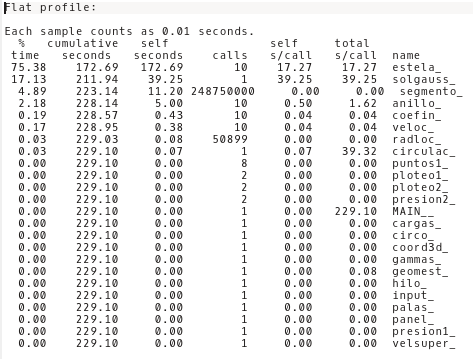
\includegraphics[width=0.60\textwidth]{figuras/gprof3.png} \\
  \caption{Resultado de \emph{gprof} en el c\'odigo optimizado serialmente.} %
   \label{figGprofInt}
\end{figure}


\subsection{An\'alisis de la subrutina Estela}

En la definici\'on de la subrutina ``estela'', el c\'odigo documentado del programa indica que \'esta realiza ``c\'alculo de los coeficientes de influencia de los hilos libres''. Los c\'alculos realizados dentro de la subrutina son numerosos y complejos, por lo cual utilizaremos un pseudoc\'odigo para poder observar los puntos m\'as importantes dentro de la subrutina que pueden ser candidatos a ser paralelizados. En la Fig. \ref{codEstela} aparece el pseudoc\'odigo anotado de la subrutina estela.

\begin{figure}[htbp]
   \begin{lstlisting}[style=consola]
    subrutina estela()
    definicion variables globales y constantes;

    begin
	Do de i=1 a 2500
	Do de j=1 a 51
		ciex(i,j) = 0
		ciey(i,j) = 0
		ciez(i,j) = 0
	end do
	end do
	%c\'alculos parciales?
	ib = 1

    Do de ir=1 a 2500
    Do de npa=1 a 51
	Do de ik=1 a 2001
		genera fx(ik), fy(ik), fz(ik), dista(ik), denom(ik)
	end do

    # sumatoria terminos impares six, siy, siz
	six,siy,siz = 0
	Do de ik=2 a 2000
		six = six + fx(ik)/denom(ik)
		siy = siy + fy(ik)/denom(ik)
		siz = siz + fz(ik)/denom(ik)
		ik = ik +2
	end do
    # sumatoria terminos pares spx, spy, spz
	spx,spy,spz = 0
	Do de ik=3 a 2000
		spx = spx + fx(ik)/denom(ik)
		spy = spy + fy(ik)/denom(ik)
		spz = spz + fz(ik)/denom(ik)
		ik = ik +2
	end do
	calculo ciex(ir,npa), ciey(ir,npa), ciez(ir,npa)
	if (indice = 1) and (ib = 1) then  ## se ejecuta solo 1 vez
	# calculo coeficientes de la estela x, y, z
		if (i = nr) and (j = nr/2) then  
		# calculo para i=50 y j=25 
		# %nr depende del tama\~no del problema,?
		# %en este caso el tama\~no es 50?
			inicializa valx,valy,valz
			Do de ik=1 a 2001
				escribe archivo integ1.txt con varios valores incluyendo valx,valy,valz
				if (ik =/= 2001) then
					const=1
					if (ik == 2000) then
						const=0.5
					endif
					valx = valx + fx(ik+1)/denom(ik+1)*otros valores
					valy = valy + fy(ik+1)/denom(ik+1)*otros valores
					valz = valz + fz(ik+1)/denom(ik+1)*otros valores
				else 
					escribe integ1.txt con varios valores sin valx,valy,valz 
					pero con ciex,ciey,ciez(i,j)
				endif
		else
			if (i = nr/2) and (j = nr+1) then 
			# Luego (si no entr\'o en el anterior if) el calculo es para i = 25 y j=51
				Repite mismo trabajo pero escribiendo integ2.txt
			endif
		endif
	endif
    end do
    end do
    end
  \end{lstlisting}
  \caption{Pseudoc\'odigo de la subrutina \emph{estela}.}
  \label{codEstela}
\end{figure}

Analizando el pseudoc\'odigo podemos observar que la subrutina tiene partes bien diferenciadas. Un inicio, estableciendo valores iniciales y c\'alculos parciales, y luego un bloque conformado por dos bucles principales; dentro de ellos es donde se encuentran las estructuras que pueden ser paralelizadas.

El bucle inicial calcula los datos en fx, fy, fz, denom y dista; luego calcula t\'erminos pares e impares, y finaliza con el denominado c\'alculo de coeficientes de la estela x,y,z. 

El c\'alculo de coeficientes parece ser el m\'as complejo de los puntos indicados, pero si observamos bien, s\'olo se ejecuta una vez en todo el programa, cuando ``indice'' es igual a 1 (la variable ``ib'' siempre tiene valor 1, por lo cual no la contamos). Dicha variable ``indice'' es global al programa y controla las etapas por las que pasa, toma valores de 1 a 10 y no repite los valores.

Por otra parte, el c\'alculo de coeficientes se hace sobre los valores valx, valy y valz, realizando sobre ellos una sumatoria, con lo cual se crea una dependencia de datos entre el c\'alculo de un valor y los c\'alculos previos (cap\'itulo 2 OpenMP), ya que para obtener el valor de valx en un momento, es necesario el valor previo de valx. Si realizamos una paralelizaci\'on del c\'odigo tendr\'iamos un problema en los l\'imites de los distintos threads. 

Por ejemplo, al dividir los datos en porciones de 100 elementos, el thread que calcula los valores 101 a 200 de un bucle necesita conocer el valor de la sumatoria en el valor 100 para poder iniciar con valores correctos su c\'alculo, y dicho valor 100 puede no existir a\'un en el momento en que se lo necesita (porque el thread encargado de su c\'alculo puede no haber finalizado o siquiera iniciado).

En el c\'alculo de los t\'erminos pares e impares se presenta el mismo problema de dependencias de datos que aparece en el c\'alculo de coeficientes. Cuando calculamos, por ejemplo, six, necesitamos conocer el valor previo de six en ese momento.

Existen t\'ecnicas y formas de transformar el c\'odigo que permiten en algunos casos poder reprogramar una porci\'on de c\'odigo para que pueda ser paralelizable a pesar de tener estas dependencias de datos. Debido al potencial gran cambio necesario en el c\'odigo para subsanar el problema de la dependencia de datos, y al requisito de no modificar el c\'odigo de maneras que puedan volverlo ilegible para el usuario, es que no se avanz\'o sobre estas \'areas de la subrutina. La soluci\'on a este problema puede ser motivo de un trabajo futuro que se pondr\'a a consideraci\'on en el cap\'itulo 5.

Luego de descartar estos puntos como las zonas a paralelizar en la subrutina ``estela'' nos quedamos con el bucle de la Fig. \ref{codEstela} que genera los arrays fx, fy, fz, denom y dista (lineas 17 a 19), ya que cada valor generado de estos arrays no depende de otros previos dentro de los arrays.

\subsection{Optimizaci\'on con OpenMP de subrutina Estela}
Seleccionado el bucle a paralelizar hicimos un an\'alisis de los datos que intervienen para poder realizar una optimizaci\'on correcta. Realizamos varias pruebas para definir las directivas OpenMP correctas, quedando definido un conjunto de datos que debe ser compartido por cada thread lanzado por OpenMP y ciertas variables que deben ser privadas de cada uno de ellos.

El bloque de c\'odigo seleccionado para optimizar es el siguiente (ha sido abreviado):
\begin{lstlisting}[style=For]
   do 3 ik=1,kult
   fx(ik)=[calculo con valores de varias matrices]
   fy(ik)=[calculo con valores de varias matrices]
   fz(ik)=[calculo con valores de varias matrices]
   fz(ik)=(-1.)*fz(ik)
   dist2=[calculo con valores de varias matrices]
   dista(ik)=dsqrt(dist2)                                  
   denom(ik)=dista(ik)**3                   
3 continue
\end{lstlisting}
Este bucle es el primer bucle interno de dos iteraciones mayores que incluyen m\'as c\'alculos con otras estructuras, las cuales dependen de los resultados obtenidos en este primer bucle.

Se calculan tres arrays llamados fx, fy y fz, un valor dist2, y dos arrays m\'as basados en el valor de dist2, llamados dista y denom.

Los c\'alculos de los tres primeros arrays y del valor dist2 dependen de varios otros arrays ya calculados previamente, y que la subrutina obtiene por el \'area de datos com\'un con el resto de partes del programa Fortran, adem\'as de utilizar funciones propias del lenguaje.

En un primer an\'alisis del bloque de c\'odigo observamos una posible dependencia de datos en las l\'ineas (5) y (8) del c\'odigo anterior. En la primera, el c\'alculo de fz(ik) depende de s\'i mismo y en la segunda el valor de denom(ik) depende del valor de dista(ik) que depende de dist2. Si bien es posible que no surgieran problemas con estos valores, para evitar resultados inesperados, decidimos analizar y modificar si fuera necesario para evitar la dependencia, siempre que el cambio no fuera significativo, como reescribir la estructura de control completa o varias l\'ineas con nuevas instrucciones.

La dependencia de datos en la l\'inea (5) pudo solucionarse r\'apida y elegantemente. La l\'inea multiplica el valor en fz(ik) por -1, por lo cual es posible agregar este c\'alculo al final de la l\'inea (4) quedando de la siguiente manera:
\begin{lstlisting}[style=For, numbers=none]
  fz(ik)=([c\'alculo con valores de varias matrices])*(-1.)
\end{lstlisting}
En el caso de la l\'inea (8) el an\'alisis es distinto: la dependencia se encuentra en el valor de dista(ik) el cual es calculado en el paso previo y depende del c\'alculo del valor dist2. Adem\'as, se trata de un c\'alculo simple con una funci\'on interna del lenguaje Fortran. Se podr\'ia utilizar un c\'alculo intermedio y luego asignar el resultado a dista(ik) y denom(ik), por ejemplo:
\begin{lstlisting}[style=For, numbers=none]
  var_aux = dsqrt(dist2)
  dista(ik) = var_aux
  denom(ik) = var_aux**3
\end{lstlisting}
Pero enfrentamos la indeterminaci\'on del valor inicial de var\_aux, y c\'omo afecta a cada bloque paralelo cuando realicemos la optimizaci\'on con OpenMP. Esto se puede resolver llevando un control de la variable en el bloque declarativo de OpenMP e inicializando la variable cada vez que es utilizada, lo que agrega carga de control al bloque de c\'odigo (tanto en OpenMP como en el c\'odigo Fortran normal). Si el c\'alculo a realizar con dist2 fuera de mayor complejidad podr\'ia justificarse la utilizaci\'on de una variable auxiliar intermedia, pero como es un c\'alculo sencillo que utiliza una funci\'on interna de Fortran a la cual se le env\'ia un solo valor, se puede resolver de la siguiente manera:
\begin{lstlisting}[style=For, numbers=none]
    dista(ik) = dsqrt(dist2)
    denom(ik) = (dsqrt(dist2))**3
\end{lstlisting}
Se puede entender mejor la dependencia de datos y la necesidad de controlar ciertas variables en los bloques paralelizados al observar un problema importante que surgi\'o durante el trabajo de tesis, el cual incluso no estaba a simple vista. 

Al realizar la optimizaci\'on paralela los resultados del programa eran distintos a los de la ejecuci\'on normal. Los resultados deben ser iguales, dado que el programa es completamente determin\'istico; por lo cual se buscaron muchas formas diferentes con directivas de OpenMP de controlar la ejecuci\'on de los threads en este bloque seleccionado para optimizaci\'on, para que los datos no se contaminaran, pero siempre arribando al mismo resultado err\'oneo. 

El problema se encontr\'o en otra porci\'on de c\'odigo que parec\'ia bastante simple de paralelizar y sin necesidad de control alguno. Al iniciar, la subrutina estela utiliza dos estructuras DO anidadas que inicializan con valor 0 tres arrays (ciex, ciey y ciez), por lo cual con una estructura OMP PARALLEL DO de OpenMP deber\'ia bastar para paralelizar el c\'alculo y obtener una mejora, si bien poco considerable, en performance.

El problema surge porque la inicializaci\'on a 0 se realiza a trav\'es de una variable llamada ``cero'' definida en otra parte del c\'odigo con el valor 0. Al lanzarse los threads de OpenMP dicha variable pas\'o a tener un valor indeterminado para cada thread, trayendo consigo datos espurios a los c\'alculos siguientes donde los arrays intervienen. Al comentar las directivas OpenMP que encerraban dichos bloques DO los resultados del programa volvieron a ser correctos.

Si bien el comportamiento por defecto de OpenMP deber\'ia ser compartir entre todos los threads las variables en memoria del programa principal, no ocurri\'o en este caso con la variable ``cero'', y no se encontr\'o una explicaci\'on para este hecho. Investigar estas particularidades, c\'omo una implementaci\'on del est\'andar OpenMP difiere de otras, y qu\'e problemas acarrean estas diferencias, puede ser motivo de una extensi\'on futura de este trabajo de tesis.  %OSO ESTO ES ASI NOMAS CHE? %HANDRU si, se quita la parte openmp y anda ok, lo arm\'e con control sobre la variable "cero" y anduvo ok, pero no lo agregue al trabajo. 

Con las modificaciones indicadas el bucle ya estaba en condiciones de ser paralelizado con OpenMP.

Lo primero que realizamos, como se planific\'o en el cap\'itulo 2, es indicar el comienzo de la regi\'on paralela y su final:
\begin{lstlisting}[style=For, numbers=none]
!$OMP PARALLEL
[bucle paralelizado]
!$OMP END PARALLEL
\end{lstlisting}
Ahora deb\'iamos agregar las directivas para indicar que la regi\'on paralela deb\'ia ser una estructura DO, por lo que agregamos las directivas DO de OpenMP:
\begin{lstlisting}[style=For, numbers=none]
!$OMP PARALLEL
!$OMP DO

[bucle paralelizado]

!$OMP END DO
!$OMP END PARALLEL
\end{lstlisting}
Al realizar estos cambios en el c\'odigo para el bloque indicado, conseguimos una gran mejora en el tiempo empleado, pero los resultados a\'un no eran correctos. Teniendo en cuenta esto debemos considerar qu\'e variables son compartidas por los distintos threads del proceso y cu\'al es su alcance, para evitar discrepancias en los resultados.

En el bloque de c\'odigo observamos que para realizar el c\'alculo de los arrays son necesarios varios otros arrays y variables, los que ya poseen valores previos. Adem\'as utiliza las variables de control ir y npa de los bloques DO exteriores donde est\'a anidado nuestro bloque de c\'odigo, utilizadas para recorrer los arrays indicados en la Fig. \ref{codEstela}. Podemos ver esto en la tabla \ref{tab:tabVar}.

\begin{table}[htb]
\begin{center}
\begin{tabular}{|c|c|}
\hline 
\rule[-1ex]{0pt}{2.5ex} Tipo Variable & Variables \\ 
\hline 
\hline
\rule[-1ex]{0pt}{2.5ex}  & pcx, pcy, pcz \\
\rule[-1ex]{0pt}{2.5ex} Arrays & xe, ye, ze \\
\rule[-1ex]{0pt}{2.5ex}  & re, fi \\
\hline
\rule[-1ex]{0pt}{2.5ex} Variable float & c0 \\
\hline
\rule[-1ex]{0pt}{2.5ex} Variables de control & ir, npa \\
\hline
\end{tabular} 
\caption{Variables necesarias para el c\'odigo paralelizado.}
\label{tab:tabVar}
\end{center}
\end{table}

El primer interrogante era saber si los datos se deben compartir entre todos los threads o deben ser privados. Si observamos todos los arrays y variables externos que se utilizan para el c\'alculo, los threads deben compartir su valor; si los defini\'eramos como PRIVATE su valor ser\'ia indefinido para cada thread, y si fuera como FIRSTPRIVATE aun cuando los valores fueran correctos, la cantidad de recursos necesarios para la ejecuci\'on se multiplicar\'ia por la cantidad de threads que estuvieran en ejecuci\'on, ya que cada uno tendr\'ia una copia de cada variable. 

Luego, los arrays modificados dentro del bloque son escritos por cada thread, pero cada thread accede a las posiciones definidas por la variable de control del bloque DO que estamos paralelizando, ik, la cual tendr\'a un valor para cada thread espec\'ifico; por ejemplo si dividimos un DO de 100 iteraciones en 2 threads, la variable de control ik tendr\'a valor inicial de 0 para un thread y 50 para el otro.

Esto nos lleva a que los arrays modificados dentro del bloque tambi\'en puedan ser compartidos por todos los threads, ya que s\'olo son accedidos indexados por la variable ik la cual, como indicamos, ser\'a distinta para cada thread, con lo cual cada uno acceder\'a a modificar posiciones de los arrays distintas.

Por todo esto, concluimos que la gran mayor\'ia de arrays y variables son compartidas por todos los threads, y la dependencia de datos entre \'estos es inexistente (los arrays escritos no son le\'idos, los arrays y variables le\'idas no son modificadas), con lo cual definimos en la instrucci\'on OpenMP de inicio del bloque paralelo como DEFAULT(SHARED) para todas las variables utilizadas dentro. Si bien \'este es el comportamiento por defecto que asume el est\'andar OpenMP, lo dejamos declarado expl\'icitamente, no s\'olo por legibilidad, sino para evitar que una eventual implementaci\'on de OpenMP de un compilador genere resultados incorrectos, por ejemplo como ocurre con la variable ``cero'' que vimos en el problema explicado previamente en esta misma secci\'on. Definimos entoncs el bloque de c\'odigo paralelo de la siguiente manera: %OSO SE ACLARO AL DESCRIBIR OPENMP QUE ES POSIBLE UNA ELECCION DE SHARING DEFAULT? HANDRU EST\'a ACLARADO
\begin{lstlisting}[style=For, numbers=none]
!$OMP PARALLEL DEFAULT(SHARED)
!$OMP DO

[bucle paralelizado]

!$OMP END DO
!$OMP END PARALLEL
\end{lstlisting}
Con esta definici\'on tenemos que todas las variables (arrays y variables comunes) ser\'an compartidas por todos los threads. 

En un siguiente nivel de an\'alisis, vemos que hay variables que necesitan definirse privadas de cada thread, principalmente la variable dist2 que es calculada dentro de cada thread en cada una de las iteraciones. Si fuera una variable compartida, todos los threads escribir\'ian en ella en orden impredecible, llevando a resultados err\'oneos. S\'olo para ejemplificar, supongamos que el thread 1 calcula la variable dist2 en una iteraci\'on, luego escribe el valor de dista(ik) con dist2; en ese momento el thread 4 calcula y escribe dist2. Cuando el thread 1 va a escribir el valor de denom(ik), dist2 ya tiene un valor completamente distinto al que hab\'ia calculado el thread 1 previamente. Por esto declaramos a dist2 como PRIVATE.

Para evitar un problema similar al de la variable ``cero'' decidimos declarar las variables de control ir y npa, y la variable ncapa como FIRSTPRIVATE, de manera que sean privadas de cada thread y tengan desde el principio su valor original. El c\'odigo resultante es el siguiente:
\begin{lstlisting}[style=For, numbers=none]
!$OMP PARALLEL DEFAULT(SHARED)
!$OMP DO FIRSTPRIVATE(ir,npa,ncapa) PRIVATE(dist2)

[bucle paralelizado]

!$OMP END DO
!$OMP END PARALLEL
\end{lstlisting}
Luego de estos cambios, la ejecuci\'on del nuevo c\'odigo dio resultados correctos comparados con la ejecuci\'on original. De esta manera paralelizamos parte del bloque de c\'odigo que m\'as tiempo consum\'ia de toda la aplicaci\'on. En el cap\'itulo 4 consideraremos la comparaci\'on de tiempos obtenidos para cada uno de los c\'odigos y soluciones a peque�os contratiempos encontrados.
